\chapter*{Januar}

2023 begann spannend. Bild \ref{fig:tomate1} zeigt ein paar Tomaten. Sie sind rot und lecker.

\begin{figure}[h!]
  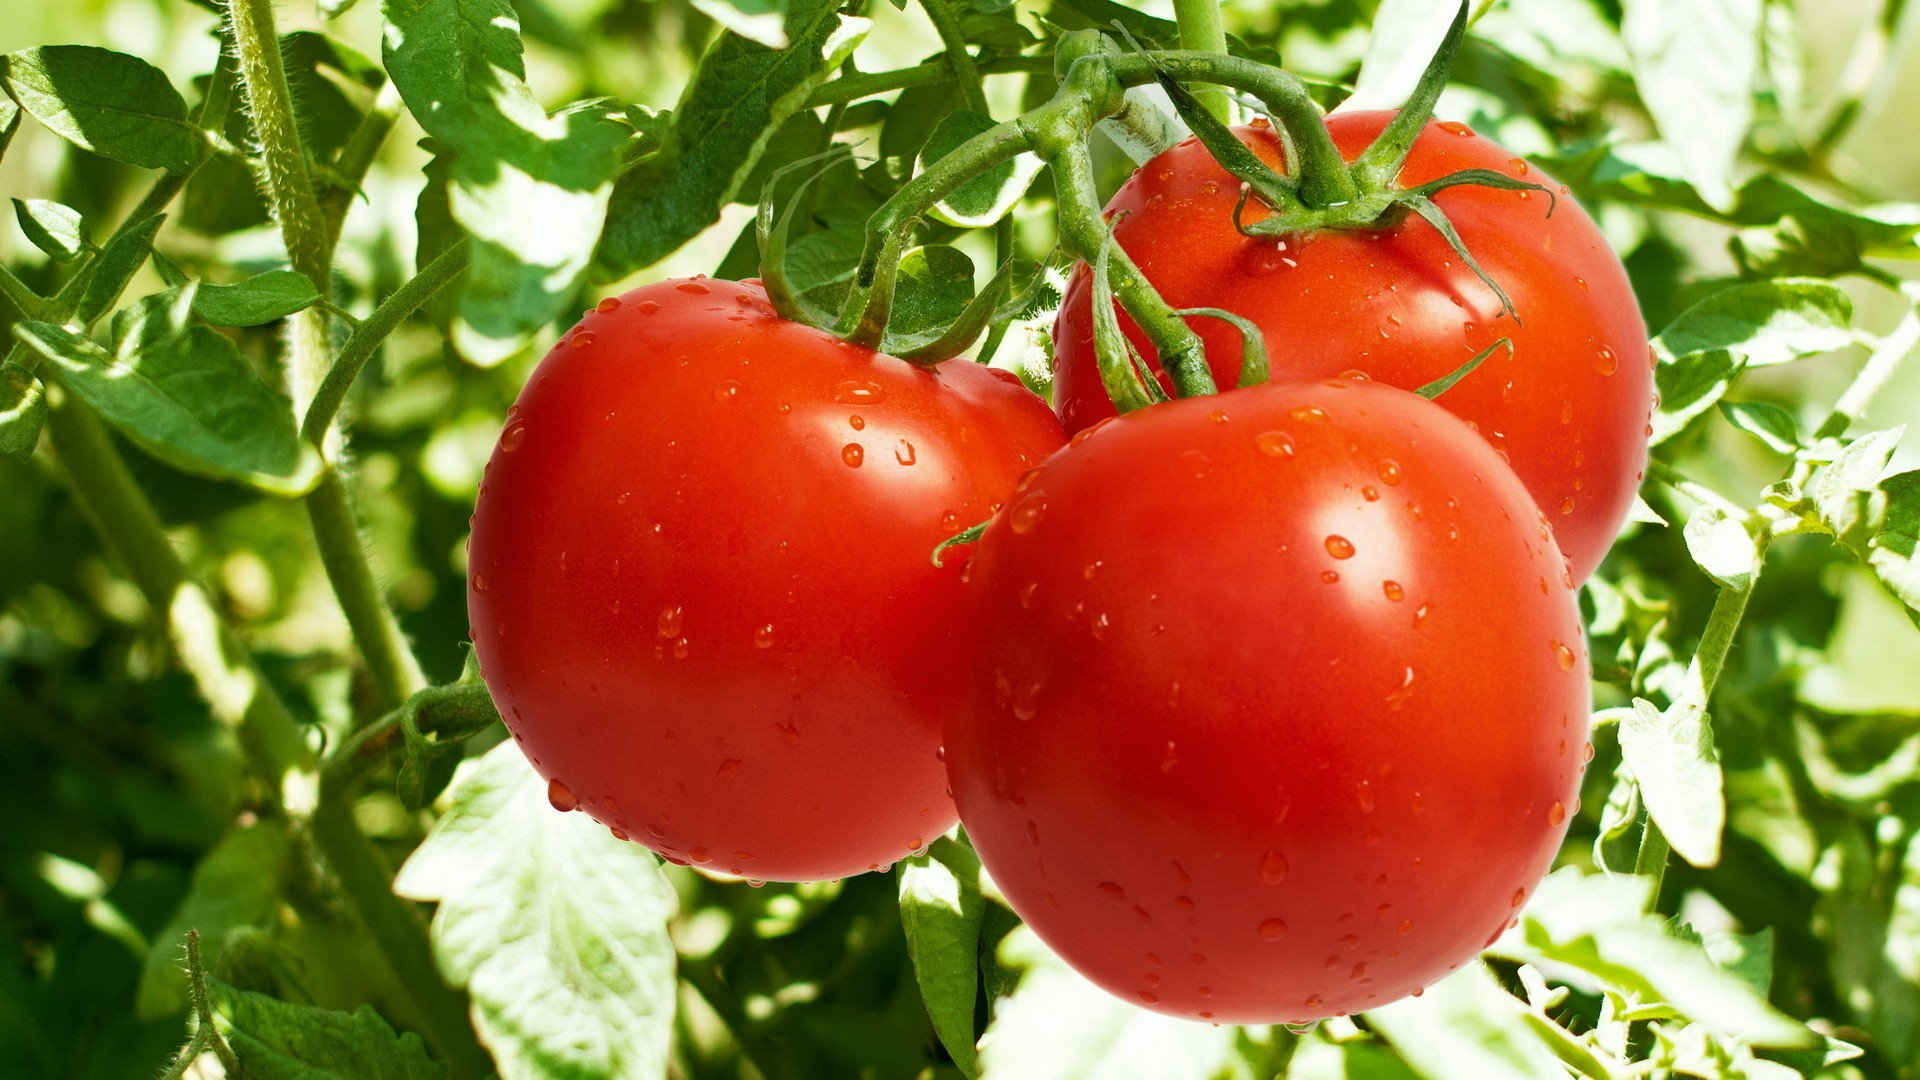
\includegraphics[width=\linewidth]{fig/tomate.jpg}
  \caption{Eine Tomate}
  \label{fig:tomate1}
\end{figure}

Ein neuer Absatz. Nochmal Tomaten, diesmal aber nebeneinander. Folgende beide Abbildungen \ref{fig:tomaten} zeigen jeweils die gleiche Tomate.

\begin{figure}[h!]
  \centering
  \begin{subfigure}[b]{0.4\linewidth}
    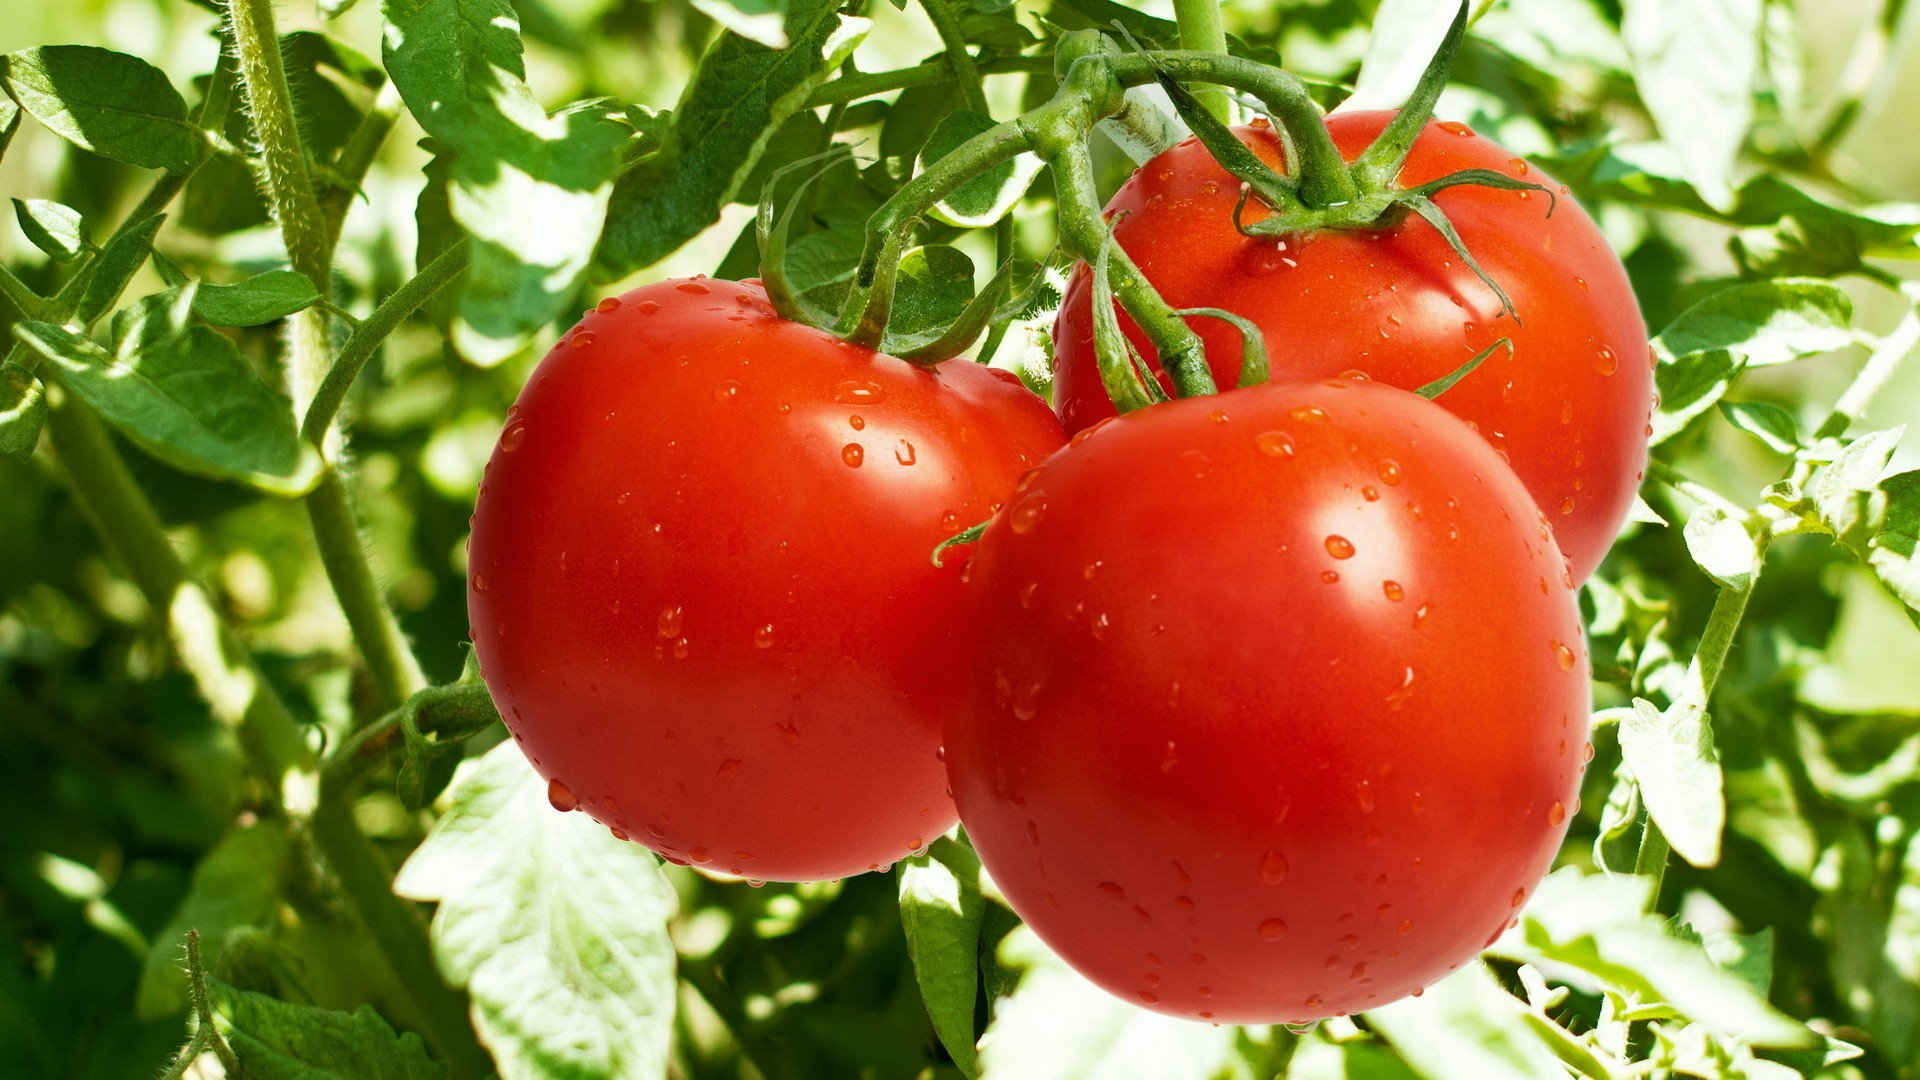
\includegraphics[width=\linewidth]{fig/tomate.jpg}
    \caption{eine Tomate}
  \end{subfigure}
  \begin{subfigure}[b]{0.4\linewidth}
    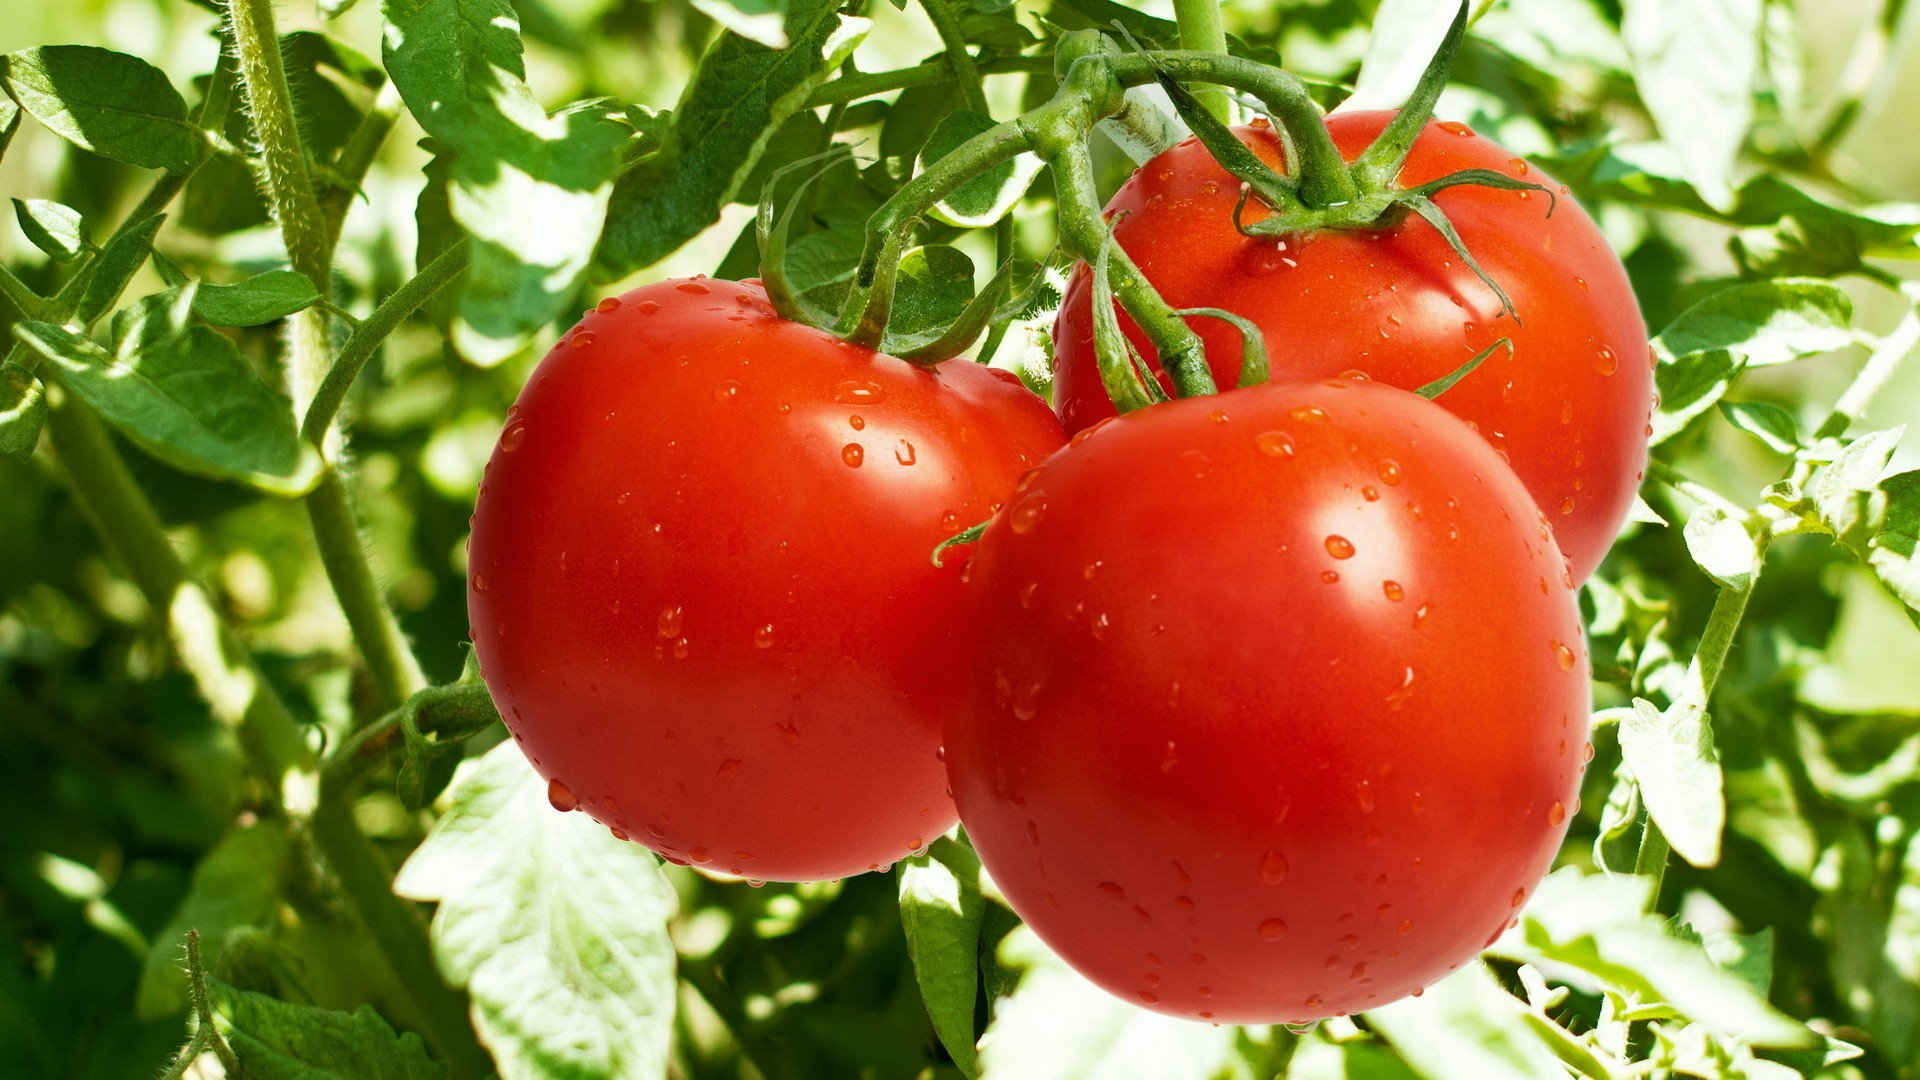
\includegraphics[width=\linewidth]{fig/tomate.jpg}
    \caption{Noch eine Tomate}
  \end{subfigure}
  \caption{Zweimal Tomate. Verrückt.}
  \label{fig:tomaten}
\end{figure}
